\sezione{4}{Esempio maschi/femmine «a conteggio»}{20–22}

È il primo esempio completo. La stima è volutamente \textbf{grossolana}: serve a vedere il meccanismo; nel resto della lezione verrà sostituita da tecniche più rigorose.

\subsection{Il problema}
\begin{minipage}[c]{.52\linewidth}\raggedright
\begin{itemize}
  \item Classificare una persona come maschio o femmina a partire da \textbf{peso e altezza}: $d=2$.
  \item $W=\{w_1=\text{maschi (blu)},\;w_2=\text{femmine (rosso)}\}$.
  \item Training set: 18 persone etichettate, \textbf{8 blu} e \textbf{10 rosse}.
  \item $\x$ (grigio) è la nuova persona; attorno a lei si considera un \textbf{intorno} (il cerchio).
\end{itemize}
\end{minipage}\hfill
\begin{minipage}[c]{.45\linewidth}
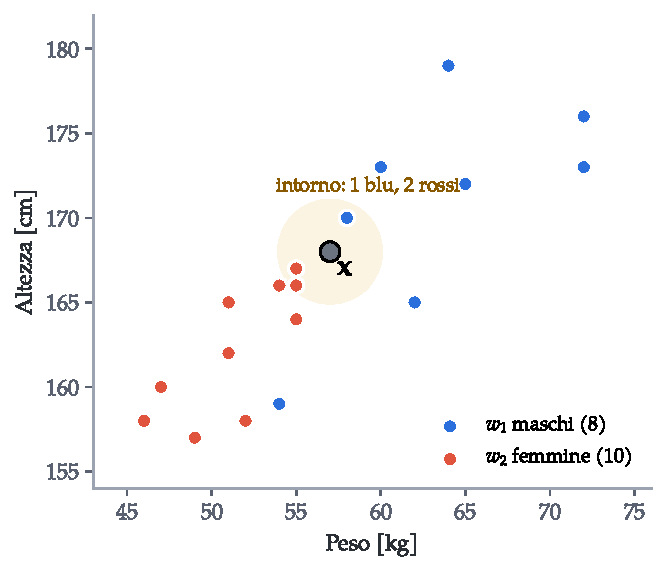
\includegraphics[width=\linewidth]{figs/conteggio.pdf}
\end{minipage}
\didascalia{Dati reali della slide 54; il pattern $\x=(57,\,168)$ ha nel cerchio 1 maschio e 2 femmine.}

\subsection{Il calcolo in quattro passi}
\begin{esempio}[Passo 1: prior]
Si contano gli esempi di ciascuna classe e si divide per il totale: $\;P(w_i)\approx n_i/n$.
\[
P(w_1)=\frac{8}{18}\approx0.44\qquad\qquad P(w_2)=\frac{10}{18}\approx0.56
\]
\end{esempio}
\begin{esempio}[Passo 2: densità condizionali]
Si contano i punti di ciascuna classe nel cerchio, in proporzione al \emph{totale della classe}:
\[
p(\x\,|\,w_1)\approx\frac{k_1}{n_1}=\frac18\qquad\qquad p(\x\,|\,w_2)\approx\frac{k_2}{n_2}=\frac{2}{10}=\frac15
\]
Si divide per $n_i$ e non per 18 perché è una probabilità \emph{condizionata alla classe}: l'universo è solo la classe $w_i$.
\end{esempio}
\begin{esempio}[Passo 3: densità assoluta]
\[
p(\x)=\frac18\cdot\frac{8}{18}+\frac15\cdot\frac{10}{18}=\frac1{18}+\frac2{18}=\frac3{18}=\frac16
\]
Lettura: 3 delle 18 persone cadono nel cerchio. La formula «complicata» conta i punti nel cerchio sul totale.
\end{esempio}
\begin{esempio}[Passo 4: posteriori e decisione]
\[
P(w_1\,|\,\x)=\frac{1/18}{1/6}=\frac13\qquad\qquad P(w_2\,|\,\x)=\frac{2/18}{1/6}=\frac23\qquad\Rightarrow\qquad \x\to w_2\ \text{(femmina)}
\]
Confidenza del 67\%. Per \emph{decidere} bastava confrontare $1/18$ e $2/18$.
\end{esempio}

\subsection{Il trucco nascosto: la posteriori è una proporzione}
Nel cerchio c'è 1 blu su 3 punti e $P(w_1|\x)=1/3$; ci sono 2 rossi su 3 e $P(w_2|\x)=2/3$. Non è un caso:
\begin{formulat}{Stima a conteggio}
$\displaystyle p(\x|w_i)\,P(w_i)=\frac{k_i}{n_i}\cdot\frac{n_i}{n}=\frac{k_i}{n}
\qquad\Longrightarrow\qquad
P(w_i\,|\,\x)=\frac{k_i/n}{k/n}=\frac{k_i}{k}$
\end{formulat}
dove $k$ è il numero totale di punti nel cerchio. Gli $n_i$ si semplificano e la regola diventa «guarda i vicini e scegli la classe più rappresentata».

\begin{mlbox}
È esattamente l'idea del \textbf{k-Nearest Neighbors (k-NN)}: il k-NN è un classificatore bayesiano «travestito», in cui le densità sono stimate in modo non parametrico.
\end{mlbox}

\subsection{Precisazione: $1/8$ non è davvero una densità}
\begin{tecnica}
Tecnicamente $1/8$ è una \emph{probabilità}: quella che un maschio cada nel cerchio. Per avere una vera densità si divide per l'area (il volume) $V$ del cerchio, come si divide una massa per un volume per ottenere la densità fisica:
\[
p(\x\,|\,w_i)\approx\frac{k_i}{n_i\,V}
\]
Il risultato del prof resta corretto perché $V$ è lo \textbf{stesso} per entrambe le classi e si semplifica nella formula di Bayes. Questa formula è il punto di partenza dell'approccio non parametrico (\emph{Parzen Window}).
\end{tecnica}

\subsection{Perché la stima è «grossolana»}
\begin{attenzione}[Limiti del metodo]
\begin{itemize}
  \item \textbf{Dipende dal raggio}: un cerchio più grande può ribaltare la decisione, uno più piccolo può essere vuoto ($0/0$).
  \item \textbf{Instabile con pochi dati}: con 1 e 2 punti, una persona in più cambia molto le stime.
  \item \textbf{Maledizione della dimensionalità}: con molte feature i cerchi restano quasi vuoti.
  \item Bisogna \textbf{conservare tutto il training set} e ricontare per ogni nuovo $\x$.
\end{itemize}
\end{attenzione}
\textbf{Effetto del prior.} Con classi equiprobabili: $P(w_2|\x)=0.2/(0.125+0.2)\approx0.62$ invece di $0.67$. Stessa decisione, confidenza un po' più bassa. Nella sezione 11 lo \emph{stesso} esempio è risolto con le gaussiane.

\begin{appunti}{— Sezione 4}
\pag{20} $d=2$ (peso, altezza); 18 esempi: 8 maschi ($w_1$, blu), 10 femmine ($w_2$, rosso). Il cerchio è l'intorno per stimare le densità.
\pag{21} Prior: $P(w_i)\approx n_i/n=8/18,\ 10/18$ (training set rappresentativo, altrimenti classi equiprobabili). Likelihood: $k_i/n_i=1/8,\ 1/5$. Densità vera: $k_i/(n_iV)$, ma $V$ si semplifica. $p(\x)=3/18=1/6$.
\pag{22} $P(w_1|\x)=1/3$, $P(w_2|\x)=2/3$ $\Rightarrow$ \textbf{femmina}. Scorciatoia: $P(w_i|\x)=k_i/k$ $\Rightarrow$ logica del k-NN. Prior uguali: $0.62$. Limiti: raggio, pochi dati, dimensionalità, memoria.
\end{appunti}
